% ============== Physik-Grundkurs Template (helles stählerndes Blau, XeLaTeX/LuaLaTeX) ==============
\documentclass[11pt,a4paper,oneside]{article}

% -------------------- Engine & Fonts --------------------
\usepackage{fontspec}
% Hauptschrift: sachlich, technisch (falls nicht installiert, fällt TeX auf Systemschrift zurück)
%\setmainfont{Fira Sans}[Scale=MatchLowercase]
%\setsansfont{Fira Sans}
\usepackage{unicode-math}
\setmathfont{Libertinus Math}

% -------------------- Pakete --------------------
%% --- Sprachen und Kodierung ---
\usepackage[ngerman]{babel}   % deutsche Sprachunterstützung
\usepackage{csquotes}         % korrekte Anführungszeichen

% --- Mathematik ---
\usepackage{amsmath}          % grundlegende Mathematikumgebung
\usepackage{mathtools}        % Erweiterungen für amsmath
\usepackage{physics}          % nützliche Makros für Physik
\usepackage{dsfont}           % Mengensymbole (z. B. \mathds{R})

% --- Schriften ---
% für XeLaTeX/LuaLaTeX: fontspec, unicode-math und Libertinus
\usepackage{fontspec}
\usepackage{unicode-math}
\setmainfont{Libertinus Serif}
\setsansfont{Libertinus Sans}
\setmonofont{Libertinus Mono}
\setmathfont{Libertinus Math}

% --- Layout und Typografie ---
\usepackage[top=3cm, bottom=3cm, left=2.5cm, right=2.5cm]{geometry}
\usepackage{microtype}        % schönerer Randausgleich
\usepackage[onehalfspacing]{setspace} % 1,5-facher Zeilenabstand
\usepackage{tocloft}          % Inhaltsverzeichnis anpassen
\renewcommand{\cftsecleader}{\cftdotfill{\cftdotsep}} 

% --- Farben und Boxen ---
\usepackage{xcolor}
\newcommand{\ricardo}[1]{%
	\colorbox{ForestGreen}{\color{white}\textsf{\textbf{Ricardo}}}%
	\textcolor{ForestGreen}{#1}%
}

% --- Tabellen und Listen ---
\usepackage{tabularx}
\usepackage{longtable}
\usepackage{dcolumn}
\usepackage{adjustbox}

% --- Grafiken ---
\usepackage{graphicx}
\usepackage{here}
\usepackage{floatflt}     % Bilder im Fließtext (eher alt)
\usepackage{epsfig}       % alte EPS-Unterstützung
\usepackage{epstopdf}     % Konvertierung EPS -> PDF

% --- Zitate und Literatur ---
\usepackage{cite}
\usepackage{bibgerm}      % deutsche BibTeX-Stile (alt; besser biblatex)

% --- Sonstiges ---
\usepackage{acro}         % Abkürzungsverzeichnis
\usepackage{blindtext}
\usepackage{lipsum}
\usepackage{listings}     % Quellcode
\usepackage{lettrine}     % Initialen
\usepackage[cute inductors,siunitx]{circuitikz} % Schaltpläne

\usepackage{amsmath}
\usepackage[ngerman]{babel}
\usepackage{acro}
\usepackage{microtype}
\usepackage{geometry}
\usepackage{titlesec}
\usepackage{fancyhdr}
\usepackage{xcolor}
\usepackage{pagecolor}
\usepackage[most]{tcolorbox}
\tcbuselibrary{skins,breakable,theorems}
\usepackage{enumitem}
\usepackage{caption}
\usepackage{everypage}
\usepackage{graphicx}
\usepackage{float}
\usepackage{wrapfig}
\usepackage{caption}
% -------------------- Tikz --------------------
\usepackage{tikz}
\usetikzlibrary{decorations.pathreplacing} % für geschweifte Klammern
\usetikzlibrary{shadings,shadows,calc}

% --------------------PGF Plots ---------------------




% -------------------- Layout --------------------
\geometry{
	left=28mm, right=28mm, top=28mm, bottom=28mm,
	marginparwidth=36mm, marginparsep=6mm
}

% -------------------- Farben (helles stählerndes Blau, dezenter Verlauf) --------------------
\definecolor{PageBGTop}{RGB}{225,233,241}   % sehr helles Stahlblau oben
\definecolor{PageBGBot}{RGB}{245,250,255}   % fast weiß-blau unten
\definecolor{BodyText}{RGB}{28,38,48}       % dunkles Schiefergrau für Text
\definecolor{AccentSteel}{RGB}{100,149,237} % steel/cornflower blue Akzent
\definecolor{AccentSky}{RGB}{150,200,255}   % helleres Blau
\definecolor{AccentWarn}{RGB}{255,120,55}   % Warnorange
\definecolor{BoxInner}{RGB}{250,253,255}    % fast weiß für Boxmitte
\definecolor{MarginalGray}{RGB}{120,130,140}

\definecolor{AccentBlue1}{RGB}{200,220,255}   % sehr helles Blau
\definecolor{AccentBlue2}{RGB}{140,170,230}   % mittelhell
\definecolor{AccentBlue3}{RGB}{80,120,200}    % dunkleres Blau
\definecolor{AccentBlue4}{RGB}{40,70,130}     % sehr dunkel
\definecolor{AccentBlack}{RGB}{25,25,35}      % fast schwarz

\definecolor{TextCream}{RGB}{250,250,245}     % helle Schrift
\definecolor{TextDark}{RGB}{30,30,40}         % dunkle Schrift
\definecolor{BoxBackground}{RGB}{255,255,255}% farblos/weiß

\definecolor{AccentSteelDark}{RGB}{50,90,160}   % dunkles Stahlblau für Section
\definecolor{AccentSteel}{RGB}{80,130,220}     % mittleres Blau für Subsection
\definecolor{AccentSky}{RGB}{150,200,255}      % helles Blau für Subsubsection



% Setze Seitenhintergrund mit TikZ-Gradient (funktioniert mit Xe/LuaLaTeX)
\pagecolor{white} % temporär; wir zeichnen Gradient mit TikZ auf jeder Seite
\AddEverypageHook{%
	\begin{tikzpicture}[remember picture,overlay]
		\shade[left color=PageBGTop,right color=PageBGBot] (current page.north west) rectangle (current page.south east);
	\end{tikzpicture}
}

% Textfarbe
\color{BodyText}

% -------------------- Kopf / Fuß --------------------
\pagestyle{fancy}
\fancyhf{}
\renewcommand{\headrulewidth}{0pt}
\setlength{\headheight}{18pt}
%\fancyhead[L]{\sffamily\small Grundkurs Physik\quad -- \quad Skript}
\fancyfoot[C]{\scriptsize\sffamily Ferdinand-Braun Schule \quad • \quad Grundkurs Physik \quad • \quad \thepage}
\fancyfoot[R]{\begin{tikzpicture}[remember picture,overlay]
		\draw[line width=0.8pt,color=AccentSteel!60!black] ($(current page.south west)+(28mm,20mm)$) -- ($(current page.south east)+(-28mm,20mm)$);
\end{tikzpicture}}

% -------------------- Titel-Styles (harmonischer Blauverlauf) --------------------
\titleformat{\section}{\normalfont\large\bfseries\sffamily\color{AccentSteelDark}}{\thesection}{1em}{}
\titleformat{\subsection}{\normalfont\normalsize\bfseries\sffamily\color{AccentSteel}}{\thesubsection}{0.8em}{}
\titleformat{\subsubsection}{\normalfont\normalsize\bfseries\sffamily\color{AccentSky}}{\thesubsubsection}{0.6em}{}


% ========================= TCBOX BASIS-STIL (physikalische, helle Boxen mit Verlauf) =========================
\tcbset{
	mybase/.style={
		enhanced,
		breakable,
		boxrule=0.9pt,
		colframe=black!20,
		colback=BoxBackground,      % Hintergrund farblos
		colupper=TextDark,
		arc=1mm,
		boxsep=5pt,
		left=15pt,right=15pt,top=15pt,bottom=15pt,
		before skip=8pt, after skip=8pt,
		attach boxed title to top left={yshift=-0.25mm-\tcboxedtitleheight/2, xshift=10mm},
		boxed title style={
			arc=3mm,
			left=6pt,right=6pt,top=3pt,bottom=3pt,
			boxrule=0pt
		},
		fonttitle=\sffamily\bfseries\small,
		title after break=\vspace{4pt}
	}
}

% -------------------- THEOREM (theo) --------------------
\newtcolorbox[auto counter,number within=section]{theo}[2][]{%
	mybase,
	colframe = AccentBlue1!80!black,
	colbacktitle = AccentBlue1!95!black,
	coltitle = TextDark,
	title = {Theorem~\thetcbcounter: #2},
	#1
}

% -------------------- BEISPIEL (exem) --------------------
\newtcolorbox[auto counter,number within=section]{exem}[2][]{%
	mybase,
	colframe = AccentBlue2!80!black,
	colbacktitle = AccentBlue2!95!black,
	coltitle = TextCream,
	title = {Beispiel~\thetcbcounter: #2},
	#1
}

% -------------------- AUFGABE (aufgabe) --------------------
\newtcolorbox[auto counter,number within=section]{aufgabe}[2][]{%
	mybase,
	colframe = AccentBlue3!80!black,
	colbacktitle = AccentBlue3!95!black,
	coltitle = TextCream,
	title = {Aufgabe~\thetcbcounter: #2},
	#1
}

% -------------------- LÖSUNG (loesung) --------------------
\newtcolorbox[use counter from=aufgabe]{loesung}[2][]{%
	mybase,
	colframe = AccentBlue4!85!black,
	colbacktitle = AccentBlue4!95!black,
	coltitle = TextCream,
	title = {Lösung~\thetcbcounter: #2},
	#1
}

% -------------------- Hinweis-Box --------------------
\newtcolorbox{infobox}[1][]{%
	mybase,
	colframe = AccentBlack!80!black,
	colbacktitle = AccentBlack,
	coltitle = TextCream,
	title = {Hinweis},
	#1
}

% -------------------- Experiment-Box --------------------
\newtcolorbox[auto counter,number within=section]{experiment}[2][]{%
	mybase,
	colframe = AccentBlue2!80!black,
	colbacktitle = AccentBlue2!95!black,
	coltitle = TextCream,
	title = {Experiment~\thetcbcounter: #2},
	#1
}

% ==================== Datum Makro ====================
\newcommand{\lessondate}[1]{\noindent\hfill\textcolor{MarginalGray}{\textsc{#1}} \\ \vspace{0.5cm}}

% ==================== Feines Titelblatt ====================
\newcommand{\MakeArtTitle}[4]{%
	\begin{titlepage}
		\begin{tikzpicture}[remember picture,overlay]
			\shade[left color=PageBGTop,right color=PageBGBot] (current page.north west) rectangle (current page.south east);
		\end{tikzpicture}
		\vspace*{25mm}
		\begin{center}
			{\Huge\sffamily\bfseries\color{AccentSteel} #1 \par}
			\vspace{8mm}
			{\Large\itshape\color{AccentSky} #2 \par}
			\vspace{12mm}
			{\Large\scshape\color{BodyText} #3 \par}
			\vspace{6mm}
			{\small\color{MarginalGray} #4 \par}
			\vspace{20mm}
			%
\includegraphics[width=0.6\textwidth]{2.png} % Logo: Pfad anpassen
		\end{center}
	\end{titlepage}
}

% ==================== Dokumentbeginn ====================
\begin{document}
	
	% Titelblatt
	\MakeArtTitle{Grundkurs Physik Q3 Hessen}{Skript und Übungsaufgaben}{Shamsher Singh Kalsi}{Berufliches Gymnasium — Ferdinand-Braun Schule \\ Kursleiter: Herr Dr. Frank Diegmüller}
	
	\tableofcontents
	\bigskip
	\clearpage
	
	\section{Einleitung}
	\lessondate{19.08.2025}\\
	Dieses Skript ist als leicht lesbare Sammlung von Vorlesungsnotizen, Experimentbeschreibungen und Übungsaufgaben für den Physik-Grundkurs gedacht. Es wurde die alte Duden Paetek Formel abgelöst und von dem IQB eine Einheitliche veröffentlicht. Auf moodle steht die neue Formelsammlung. Thomsoneschwingungsgleichung. 
	
	\subsection{Ablauf des Kurses}
	
	\subsubsection{Randbemerkungen}
	
	
	\newpage
	
	
	\section{Wiederholung}
	%\lessondate{19.08.2025}\\
	
	\subsection{Interferenz und Beugung am Doppelspalt}
	
	Die Überlagerung von Lichtwellen am Doppelspalt ist eines der klassischen Experimente der Wellenoptik und wurde erstmals von \textsc{Thomas Young} im Jahr 1801 durchgeführt. Es zeigt, dass Licht Welleneigenschaften besitzt, da sich charakteristische Interferenzmuster nur durch das Prinzip der Überlagerung erklären lassen. Die beobachteten Helligkeitsmaxima und -minima entstehen durch konstruktive und destruktive Interferenz zweier kohärenter Wellenzüge, die durch die beiden Spalte hindurchlaufen.
	
	
	\begin{minipage}[t]{0.45\textwidth}
		\vspace{0mm}
		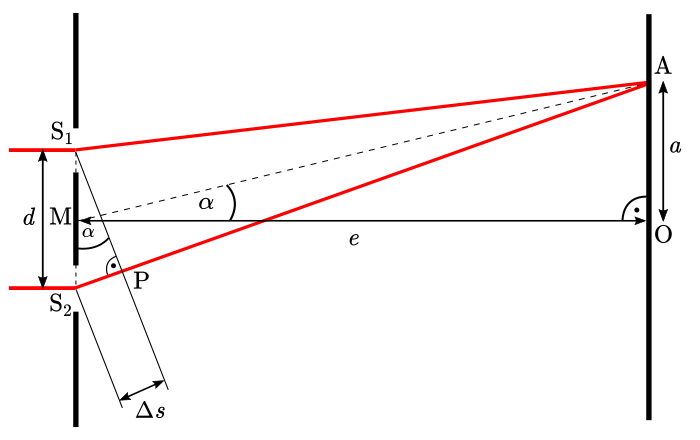
\includegraphics[width=\textwidth]{Doppelspalt_Einstiegsaufgaben_Bild.png}
		\captionof{figure}{Doppelspalt Nahaufnahme}
	\end{minipage}%
	\hfill
	\begin{minipage}[t]{0.45\textwidth}
		\vspace{0pt} % zwingt die Oberkante wirklich nach oben
		\begin{itemize}
			\item [$d:$] Abstand der Mittelpunkte der Spalten 
			\item [$e:$] Abstand zwischen Doppelspalt und Schirm 
			\item [$a:$] Abstand eines Punktes $A$ auf dem Schirm zum Punkt $O$ , an dem sich das 0. Maximum befindet
			\item [$\alpha:$] Weite des Winkels 
		\end{itemize}
	\end{minipage}

	Die Bedingung für konstruktive Interferenz lautet
	\begin{align*}
		\sin \alpha &= \frac{k \cdot \lambda}{d}, \quad k \in \mathbb{Z},
	\end{align*}
	wobei $k$ die Ordnung des Maximums bezeichnet. Für destruktive Interferenz ergibt sich entsprechend
	\begin{align*}
		\sin \alpha &= \frac{(2k - 1)\cdot \frac{\lambda}{2}}{d}, \quad k \in \mathbb{N}.
	\end{align*}
	
	Für kleine Winkel $\alpha$ kann man näherungsweise $\sin \alpha \approx \tan \alpha \approx \frac{a}{e}$ setzen, sodass die Position $a$ der Maxima auf dem Schirm berechnet werden kann:
	\begin{align*}
		a_k \approx \frac{e \cdot k \cdot \lambda}{d}.
	\end{align*}
	
	
	\subsection*{Wichtige Wellenphänomene (vgl. Tipler, S. 493)}
	
	\begin{theo}{Definitionen grundlegender Wellenphänomene}
		\begin{enumerate}
			\item \textbf{Reflexion:} Richtungsänderung einer Welle an einer Grenzfläche, sodass sie in das Ursprungsmedium zurückkehrt (z.~B. Spiegel).
			\item \textbf{Beugung:} Ablenkung und Ausbreitung einer Welle hinter Hindernissen oder Öffnungen, die mit der Wellenlänge vergleichbar sind.
			\item \textbf{Brechung:} Änderung der Ausbreitungsrichtung einer Welle beim Übergang in ein Medium mit unterschiedlicher Ausbreitungsgeschwindigkeit.
		\end{enumerate}
	\end{theo}
	
	%\begin{figure}[h]
	%	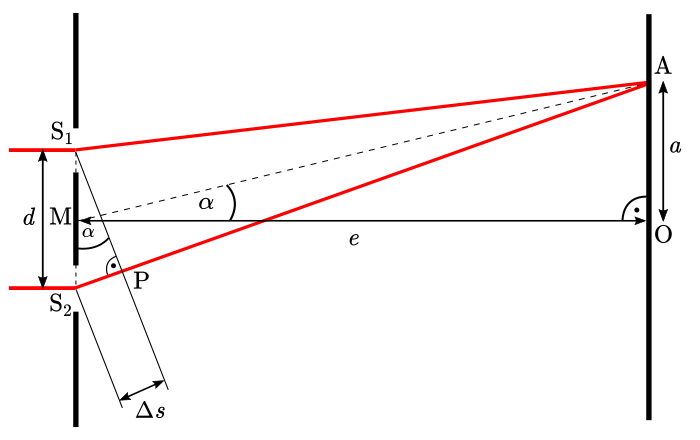
\includegraphics[width=0.5\textwidth]{Doppelspalt_Einstiegsaufgaben_Bild.png}
	%\end{figure}
	
	\newpage
	
	\section{Elektromagnetische Wellen}

	\section{Welle-Teilchen-Dualismus}
	\section{Atomvorstellungen}
	
	
	\section{Quantenobjekte}
	\section{Astrophysik}
	
	
	\newpage
	
	
	\section{Mechanik}
	
	\section{Elektrizitätslehre}
	
	\section{Optik}
	
	\section{Thermodynamik}
	
	\newpage
	
	
	
	
	
	% Beispiel-Boxen
	\begin{theo}
		In einem abgeschlossenen System bleibt die Gesamtenergie erhalten.
	\end{theo}
	
	\begin{exem}{Körper im Schwerefeld}
		Ein Körper der Masse $m$ wird aus der Höhe $h$ fallen gelassen. Seine potentielle Energie ist $E_p = mgh$.
	\end{exem}
	
	\begin{aufgabe}{Freier Fall}
		Berechne die Aufprallgeschwindigkeit eines Körpers nach einer Fallhöhe $h$ (ohne Luftwiderstand).
	\end{aufgabe}
	
	\begin{loesung}{Skizze}
		Mit Energieerhaltung: $\frac12 mv^2 = mgh \Rightarrow v=\sqrt{2gh}$.
	\end{loesung}
	
	\begin{infobox}{Sicherheit}
		Trage Schutzbrille bei Experimenten mit Spritzgefahr.
	\end{infobox}
	
\end{document}
